

\section{Python interpreters}\label{sec:pythoninterpreters}

%%% note : add this to the section of python interpreters 
Due to the lack of of support for most of  non conventional pyton interpeters, our main focus was only on micro benchmarks.
Except pypy most of the python implementations don't support extra python libraries, Despite that most of the cases those extra implementations were made to optimize a specific library such as numba with numpy, or intelpython with machine learning algorthms.

\paragraph{preliminary studies}
For the first studies we used only the official version of python. because the goal was mainly to highlight the impact of the structure of code on the energy consumption.
One main inconvienent of the previous methode to reduce the energy consumption, is the hard work that should be done in order to alter the existing code base in order to redcue the energy consumption. To avoid such hustle we tried to find a non intrusive way to make the python code more ecofriendly without changing its structure. One aspect of python is the fact that it is an interptered language which led many works to create their own implementation of the interpeter to enhance one or many aspect of the python code. in the following section we will discuss the impact of those implementations on the energy consumption of python programs, and in which case, one should use a non conventional interpter to save the energy consumption of their program.

To do so, we gathered a list of interpeters, transpilers and some optimization libraries.

the following list, presents the most famous ones .
% We should explain the methodology we used to select these

\begin{enumerate}
    \item \textbf{CPython}:\footnote{\url{https://www.python.org/}} a Python interpreter written in C programming language. It is the reference interpreter of Python. CPython compiles the source code into a bytecode and then interprets it. The CPython project still supports both versions of Python 2 and 3;
    \item \textbf{PyPy}:\footnote{\url{http://pypy.org}} An alternative implementation of the Python interpreter. It is written using \emph{RPython} in order to use the JIT. It compiles the most used portions of the Python code into a binary code for better performance. To benefit from these optimizations, the program has to be executed for at least for few seconds so the JIT has enough time to warm up, the JIT optimization will be applied only the code written by the programmer and not external libraries;
    \item \textbf{Cython}:\footnote{\url{https://github.com/cython/cython}} a static compiler for Python. It translates the Python code into a C code, and then compiles it using a C compiler. It also support(s) an extended version of the Python language that allows programmers to call \emph{C functions}, declare \emph{C types} and use static types which will help the translation of Python objects into native types, such as integers, float, which often means a better performances, since native C libraries are almost all the time faster than the python written once~\cite{pereira_energy_2017}.
    \item \textbf{Intel\,Python}:\footnote{\url{https://software.intel.com/en-us/distribution-for-python}} A customized interpreter developed by Intel in order to enhance performances of Python programs. It is dedicated to data sciences, high-Performance computing. It uses some Intel kernel libraries, such as Math Kernel Library (Intel MKL\footnote{\url{https://software.intel.com/en-us/mkl}}) and data analytics acceleration library (Intel DAAL\footnote{\url{https://software.intel.com/en-us/intel-daal}}). It supports both versions of Python;
    \item \textbf{Active\,Python}:\footnote{\url{https://www.activestate.com/products/activepython/}} developed by the Activestates company, it provides a standardized Python distribution to ensure license compliance, security, compatibility and performance. Therefore, ActivePython has its own built-in packages (more than 300 packages) and supports both versions of Python;
    \item \textbf{IronPython}:\footnote{\url{https://ironpython.net}} A .Net-based Python interpretation platform written in C\# in order to be used over the .Net vm or mono, it benefits from all the optimizations of .Net virtual machine, such as the JIT and garbage collector mechanisms.
    \item \textbf{GraalPython}:\footnote{\url{https://github.com/graalvm/graalpython/}} A Python interpreter that is based on GraalVM \footnote{\url{https://www.graalvm.org/docs/why-graal/}} (a universal virtual machine developed by oracle for running applications written in different programming languages). For the time being, it only supports Python~3 and it is still in the experimental stage;
    \item \textbf{Jython}:\footnote{\url{https://jython.github.io}} Implementation of Python programming language written in Java for the \emph{Java virtual machine} (JVM). Similar to IronPython and GraalPython, it leverages the optimization mechanisms provided by the JVM to enhance the Python programs;
    \item \textbf{MicroPython}:\footnote{\url{http://micropython.org}} a lightweight Python version dedicated to embedded systems and micro-controllers;
    \item \textbf{Nuitka}:\footnote{\url{http://nuitka.net/pages/overview.html}} a Python compiler written in Python that generates a binary executable from Python code. It translates the Python code into a C program that is then compiled into a binary executable;
    \item \textbf{Numba}:\footnote{\url{https://numba.pydata.org}} a library that includes JIT compiler in order to enhance the performances of Python functions using the industry-standard LLVM compiler library;
    \item \textbf{Shedskin}:\footnote{\url{https://github.com/shedskin/shedskin}} a static transpiler that translates implicitly statically typed python into C++ code.
    \item \textbf{Hope}~\cite{akeret_hope_2015}: a Python library that aims to introduce JIT compiler into the Python code;
    \item \textbf{Parakeet}~\cite{DBLP:conf/hotpar/RubinsteynHWS12}: a runtime accelerator for an array-oriented subset of Python;
    \item \textbf{Stackless\,Python}:\footnote{\url{https://github.com/stackless-dev/stackless/wiki}} an interpreter that focus on enhancing multi-threading programming.
    \item \textbf{Pyjion}:\footnote{\url{https://github.com/microsoft/pyjion}} JIT API for CPython, same purpose as Parakeet and Hope.
    \item \textbf{Pyston}:\footnote{\url{https://blog.pyston.org}} performance-oriented Python implementation built using LLVM and modern JIT techniques. the project is funded by dropbox;
    \item \textbf{Grumpy}:\footnote{\url{https://github.com/google/grumpy}} a source-to-source transpiler that translates the Python code into a Go code that will be compiled to a binary executable. It also offers an interpreter called \emph{grumprun} which can directly execute the Python code. Unfortunately, we cannot use it because the project is already outdated (last commit is in 2017) and it has a lot of limitation in term of supporting the Python language, such as some built-in functions and standard libraries;
    \item \textbf{Psyco}:\footnote{\url{http://psyco.sourceforge.net}} a JIT compiler for Python;
    \item \textbf{Unladen\,Swallow}:\footnote{\url{https://unladen-swallow.readthedocs.io/en/latest/}} an attempt to (use) LLVM  as  JIT compiler for CPython.
\end{enumerate}


\subsection{Runtime Classification}
Before futher proceeding with the list of candidate runtimes for Python applications, we propose a classification according to several criterions:
\begin{description}
    \item[\bf Type] refers to the category of runtime infrastructure that supports the execution of a Python application. In particular, we consider 3 types of environments: \emph{Interpreter}, \emph{Compiler} and \emph{Library}. \emph{Interpreter} refers to the class of environment that does not require any preprocessing of Python source code. \emph{Compiler} introduces a compilation phase prior to the execution of the application. Finally, \emph{Library} induces some modification of the source code.
    \item[\bf Runtime] refers to the technology supporting the execution of a Python application. This technology can refer to the programming language used to program the interpreter, the target language for a compiler or a library.
    \item[\bf JIT optimisation] refers to the support of \emph{just-in-time} compilation in the runtime infrastructure supporting the execution of the application.
    \item[\bf GC optimisation] refers to the support of \emph{garbage collection} in the runtime infrastructure supporting the execution of the application.
    \item[\bf Python version(s)] refers to the list of Python source code versions supported by the runtime environment.
\end{description}

We should explain the classification of these runtimes

\begin{table}
    \caption{Classification of Python implementations}
    \label{fig:python-classes}
    \center
    \begin{tabular}{|l|c|c|c|c|c|c|}
        \hline
        \multirow{2}{*}{\bf Name} & \multirow{2}{*}{\bf Type} & \multirow{2}{*}{\bf Runtime} & \multicolumn{2}{c|}{\bf Optimisations} & \multicolumn{2}{c|}{\bf Python}                     \\
        % \cline{1-5} 
                                  &                           &                              & {\bf JIT}                              & {\bf GC}                        & {\bf 2} & {\bf 3} \\
        \hline
        \hline
        CPython                   & Interpreter               & C                            & \no                                    & \no                             & \yes    & \yes    \\
        \hline
        Intel\,Python             & Interpreter               & C                            & \no                                    & \no                             & \yes    & \yes    \\
        \hline
        ActivePython              & Interpreter               & C                            & \no                                    & \yes                            & \yes    & \yes    \\
        \hline
        PyPy                      & Interpreter               & Python                       & \yes                                   & \yes                            & \yes    & \yes    \\
        \hline
        IronPython                & Interpreter               & .Net                         & \yes                                   & \yes                            & \yes    & \yes    \\
        \hline
        GraalPython               & Interpreter               & GraalVM                      & \yes                                   & \yes                            & \no     & \yes    \\
        \hline
        Jython                    & Interpreter               & Java                         & \yes                                   & \yes                            & \yes    & \no     \\
        \hline
        Stackless\,Python         & Interpreter               & python                       & \no                                    & \no                             & \yes    & \no     \\
        \hline
        MicroPython               & interpreter               & c                            & \no                                    & \no                             & \no     & \yes    \\
        \hline
        Pyston                    & interpreter               & LLVM                         & \yes                                   & \no                             & \yes    & \no     \\
        \hline
        Unladen\,Swallow          & Interpreter               & LLVM                         & \yes                                   & \no                             & \yes    & \no     \\
        \hline
        Cython                    & Compiler                  & C                            & \no                                    & \no                             & \yes    & \yes    \\
        \hline
        Nuitka                    & Compiler                  & C                            & \no                                    & \no                             & \yes    & \yes    \\
        \hline
        Shedskin                  & Compiler                  & C++                          & \no                                    & \no                             & \yes    & \yes    \\
        \hline
        Grumpy                    & Compiler                  & Go                           & \no                                    & \no                             & \yes    & \yes    \\
        \hline
        Numba                     & Library                   & C                            & \yes                                   & \no                             & \yes    & \yes    \\
        \hline
        Hope                      & Library                   & python                       & \yes                                   & \no                             & \yes    & \yes    \\
        \hline
        Psyco                     & Library                   & python                       & \yes                                   & \no                             & \yes    & \yes    \\
        \hline
        Pyjion                    & Library                   & .NET Core                    & \yes                                   & \no                             & \yes    & \yes    \\
        \hline
        Parakeet                  & library                   & C                            & -                                      & \no                             & \yes    & \no     \\
        \hline
    \end{tabular}
\end{table}



\begin{table}[hbt]
    \caption{Classification of Python implementations}
    \label{fig:pythonimplementations}
    \center
    \begin{tabular}{|l|c|c|c|}
        \hline
        Version  & Interpreter     & Transpiler/Compiler & Jit library \\
        \hline
        \hline
        Python~2 & Cpython2        & Cython2             & Numba 2     \\
        % \cline{2-4} 
                 & Pypy2           & Shesdskin           & Hope        \\
        % \cline{2-4} 
                 & Pytson          & Grumpy              & Parakeet    \\
                 & Ironpython      &                     & Psyco       \\
                 & Jython          &                     & Pyjion      \\
        % &  &  &  \\
                 & Micropython     &                     &             \\
                 & Pysec           &                     &             \\
                 & StacklessPython &                     &             \\
        % \cline{2-4} 
        \hline
        Python~3 & Cpython3        & Nuitka              & Numba3      \\
                 & Pypy3           &                     &             \\
                 & GraalPython     &                     &             \\
        \hline
    \end{tabular}
\end{table}

There are other implementations that we didn't considerate because either the project aborted many years ago or it has a very limited support for python features.
After the collection of those implementation we filtered them. in order to keep only the versions that are still maintained and support most of python features.
and we classified them into 3 categories depending of their integration with the python code.  In the \ref{fig:pythonimplementations} we describe the implementations that we kept and the version of each implementation and its category.


\begin{figure}
    \centering
    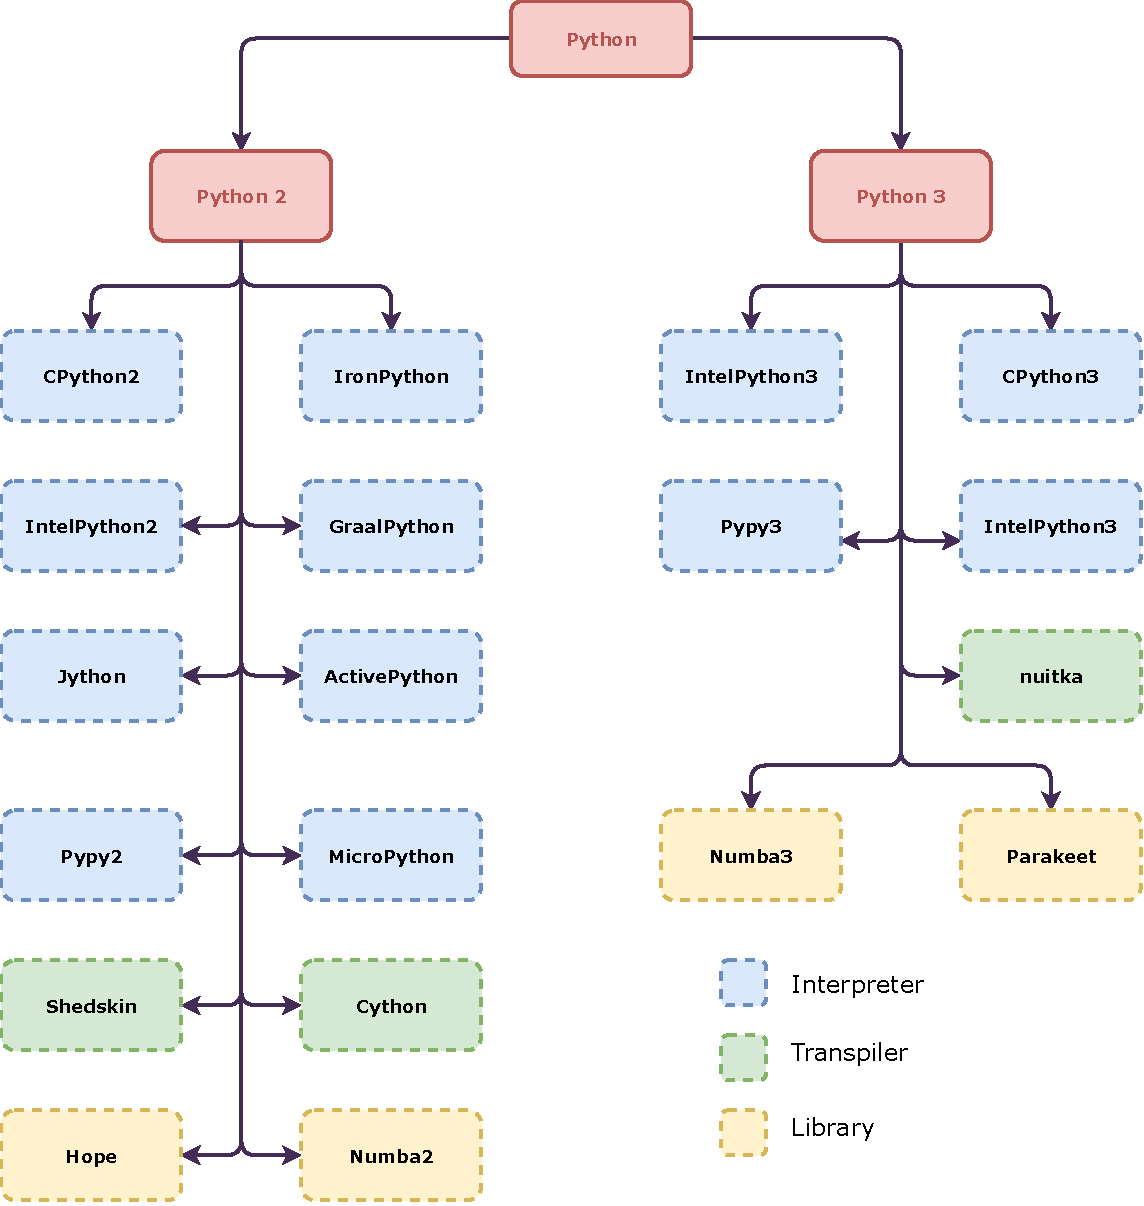
\includegraphics[width=\linewidth]{imgs/python-implementations-tree}
    \caption{Python interpeters}
    \label{fig:interpreters}
\end{figure}



\section{experimetal protocole}

As we have discussed in the previous chapter \ref{chapter:benchmarking}. instead of running the tests, the idea was to design a system that allows practiouners to reproduce and extends our tests. and then we use the same system to run answer some of researchs question.
%%%% probably ill resue the same things from other chapters 
\subsection{measurement context}
\paragraph{Hardware settings}

all our tests have been executed in a Dell PowerEdge C6420 server machine. A summary of its hardware is listed in table \ref{fig:dahuconfig}. The machine is equiped with a minimal version of Debian\,9 (4.9.0 kernel version) where we install Docker (version 18.09.5).



\begin{table}[hbt]
    \begin{tabular}{ll}
        \hline
        CPU     & Intel Xeon Gold 6130 (Skylake, 2.10GHz, 2 CPUs/node, 16 cores/CPU)                                                     \\
        Memory  & 192 GiB                                                                                                                \\
        Storage & 240 GB SSD SATA Samsung MZ7KM240HMHQ0D3                                                                                \\
                & 480 GB SSD SATA Samsung MZ7KM480HMHQ0D3                                                                                \\
                & 4.0 TB HDD SATA Seagate                                                                                                \\
        Network & eth0/enp24s0f0, Ethernet, configured rate: 10 Gbps, model: Intel Ethernet Controller X710 for 10GbE SFP+, driver: i40e \\
                & ib0, Omni-Path, configured rate: 100 Gbps, model: Intel Omni-Path HFI Silicon 100 Series [discrete], driver: hfi1      \\
        \hline
    \end{tabular}
    \caption{Testing Machine Configuration }
    \label{fig:dahuconfig}
\end{table}

\begin{figure}[hbt]
    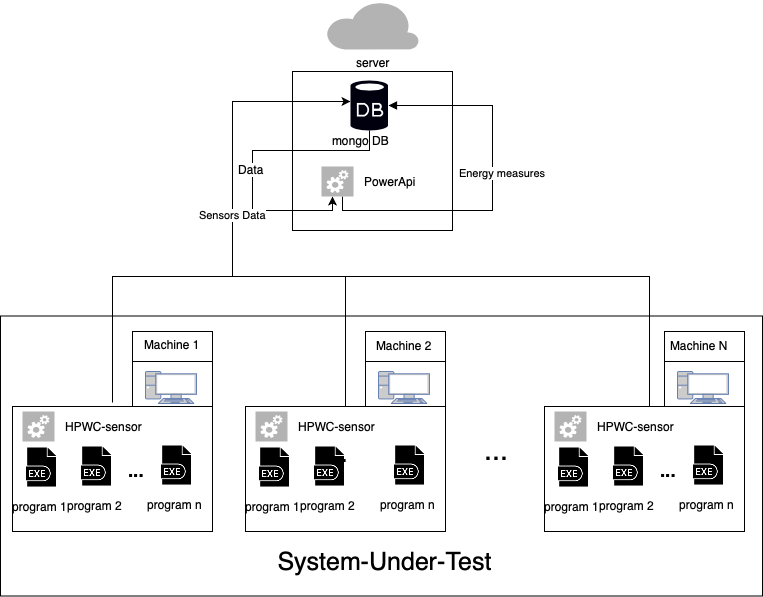
\includegraphics[width=\linewidth]{imgs/SmartWatts.png}
    \caption{powerapi architecture}
    \label{fig:powerapi}
\end{figure}

\paragraph{software settings}
For the sake of reproducibility, each experiment runs within a Docker container.
% for each test we create a docker image.
\subsection{Metrics}
Our focus will be mainly on CPU energy consumption because it is ten folds more than the DRAM one, since it is finit job benchmarking, time is highly correlated within the energy, and it will be only useful to explain certain energytical behaviour so we wont put a lot of focus on this metric.

%% basically i what i want to say is that we we care mostly about energy, because there are studies that were made on the performance, plus the DRAM is not that interested even within the heavy memory  benchmakrs 
% TODO : ADD DRAM graphs for vectors and matrix multiply 


\paragraph{Energy measurement}

As we know, the energy of a program is the integrale of its power overtime. For us ower case, we used Intel \emph{Running Power Average Limit} (RAPL)~\cite{Khan:2018:RAE:3199681.3177754} to collect the power samples of the running tests,

We used used \textsc{PowerAPI}~\cite{DBLP:journals/jss/ColmantRKSFS18}, to report Data collected by intel Rapl and send it into another machine that we call computing machine. then we calculate the Energy using  the the trapezoidal rule.


\ref{fig:trapezrule}
\begin{figure}[hbt]
    \centering
    \begin{equation}
        E = \int^a_b P(t)dt \simeq \sum^n_{k=1} \frac{P(t_k-1)+P(t_k)}{2}
    \end{equation}
    \caption{}
    \label{fig:trapezrule}
\end{figure}



figure \ref{fig:powerapi} shows the architecture of our testing model.


The reason of separation between data collection and energy calculation is to minimise any interference with the test so our sensor is a light c program running inside a docker container.
\subsection{tests preparation}



To study the behaviour of the python implementation regarding the energy consumption, we have to focus on the effect of the implementation and mitigate the maximum any side effects such as the organisation of the code or any extra consumption due to the operating system or tier libraries.
Therefore, for each test we took the implementation written in python2 as a reference and tried to use it in other implementations as it is. If it is not supported by python3, we transformed the code using the officiel library  \emph{2to3}\footnote{\url{https://docs.python.org/3.7/library/2to3.html}}.
In the case of the libraries that use \emph{JIT} adding a decorator to the function that we want to optimize was enough, if there are other changes we assume that they alter the original code which is against our purpose.

Each test is implemented in a Docker container for the several reasons
\begin{itemize}
    \item Isolation: each container has only the test program implemented with a single python runtime to remove any interference between different implementations.
    \item Deplpoyment: to use the testing machine without extra configurations that may alter the behaviour of the os toward the enrgy consumtion
    \item Reproductibility: One of the most frequent benchmark crimes~\cite{DBLP:journals/corr/abs-1801-02381} in research is the lack of Reproductibility, by using Docker we ensure that each test has an Image that will be accessible in public.
\end{itemize}

Despite the presence of the official docker images for the most of the runtimes, we prefered to build our own using the same reference image in order to remove any bias due to the Os used in the offical image.We used ArchLinux with the kernel version 4.9.184 as a base image.


\subsection{Extension}
As we have done with the previous chapters. we provide a tool that allows to extend the tests with new workloads and new candidates.
In the repository \footnote{\url{https://github.com/chakib-belgaid/python-implementations}}.
we have a tool that allows to generate new workloads and new candidates.
The script \texttt{generator.py} allows to create new benchmarks by implementing a python code within different interpeters. then it generates \texttt{launcher-benchmark.sh} that can be used directly to run the expermient. Furthermore all the successful implementations are stored in seperate directory and the that couldn't work ( mostly because of compatibility issues) stored in a recap file called \texttt{benchmarkTest.md}. where benchmark is the name of the new workload;
To add extra \textbf{candidates} one should add a base docker file
that containes the new implementation and if there should be extra manipulation that should be added to the workload files ,such as adding new decorator or changing some parameters, then they should be added as an extra function in the script \texttt{generator.py}. Finally they should be included in the python candidates.

\section{Results and finding}



\section{placeholder}
we performed a shapiro normality test for the first on the results, and almost all the p-values smaller than alpha=0.01\%
therefore the distrubution is not normal - which is kinda true because if it was normal then we dont have any comparaison --

for arrays and vectors  graalpython took so much time that we decided to remove it

the startup cost for ironpython was too high
for graalpython and ipy they couldnt handle big numbers hence the overflow  when it comes to execution time
but since we measure the energy outside the values of the energy aren't impacted

as usual there is  correlaction between DRAM and CPU so no need to classify based on DRAM + the DRAM consumes less 10\% of the  energy compared to the CPU

so the plan is to prove that there is a statistical difference
then we use the multiparameter optimization , howerver we stop in the phase where we calculate the score
because we dont know the weight of each parameter ( of tommti microbenchmark) and instead of doing the sum with the coefissients we use the radar plot to let the reader decide which one is the most suitable for his usage. howerver since the differences are gigantics we change the scale to logarithmic to be easier for the eye to read



\begin{figure}
    \caption{energy consumption of different impelementations using Bit Operation benchmarks (Joule) }
    \label{table:bitops}
    \begin{tabular}{lrrrrr}
        \toprule
        benchmark    & A          & GG         & LL         & Or         & XOR        \\
        \midrule
        activepython & 676.980672 & 763.208040 & 651.783048 & 743.016425 & 728.828481 \\
        cpython2     & 441.082298 & 435.886950 & 430.846171 & 415.247383 & 419.081447 \\
        cpython3     & 595.209019 & 685.085315 & 563.839300 & 657.972734 & 655.560574 \\
        cython       & 35.077408  & 182.688395 & 274.177830 & 34.868014  & 34.504778  \\
        nuitka       & 33.260991  & 32.980380  & 33.256450  & 33.472770  & 33.030889  \\
        numba2       & 9.102939   & 8.411176   & 9.460620   & 9.375920   & 9.755952   \\
        numba3       & 9.566646   & 10.144212  & 9.219703   & 9.344613   & 9.665108   \\
        pypy2        & 8.456867   & 7.844918   & 8.286278   & 8.138692   & 7.952999   \\
        pypy3        & 7.552731   & 8.093884   & 8.108508   & 8.669448   & 8.623737   \\
        shedskin     & 8.024198   & 8.070870   & 8.399917   & 8.126236   & 8.277546   \\
        \bottomrule
    \end{tabular}

\end{figure}


\begin{figure}
    \centering
    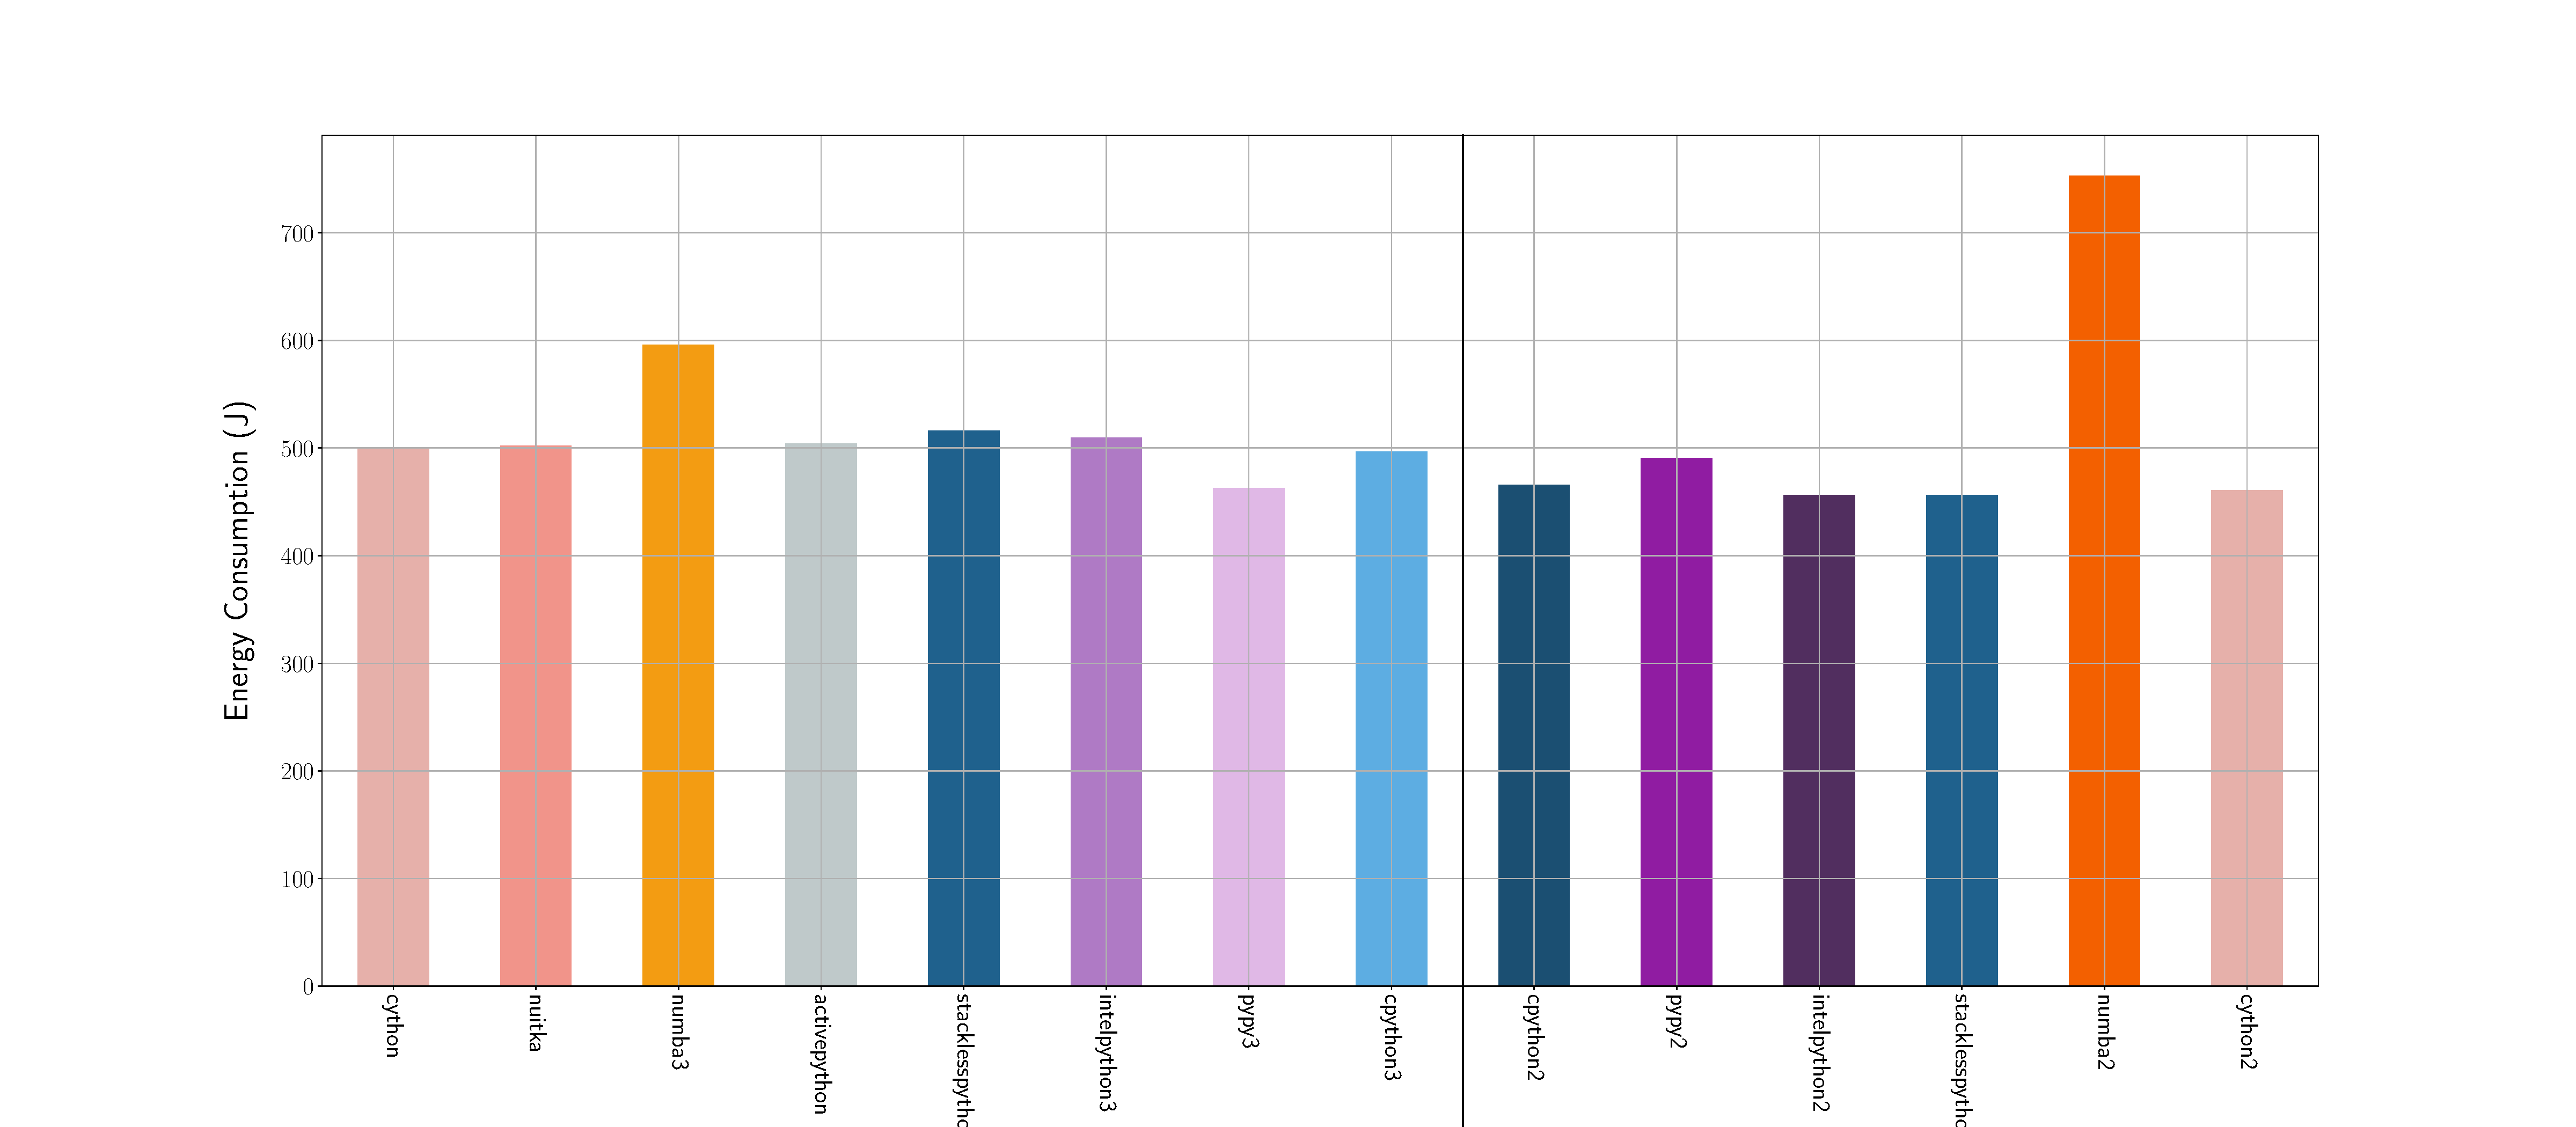
\includegraphics[width=\linewidth]{imgs/barplot_binarry_tree}
    \caption{energy behaviour based on multiprocessing}
    \label{fig:python_multiprocessing}
\end{figure}

\begin{figure}
    \centering
    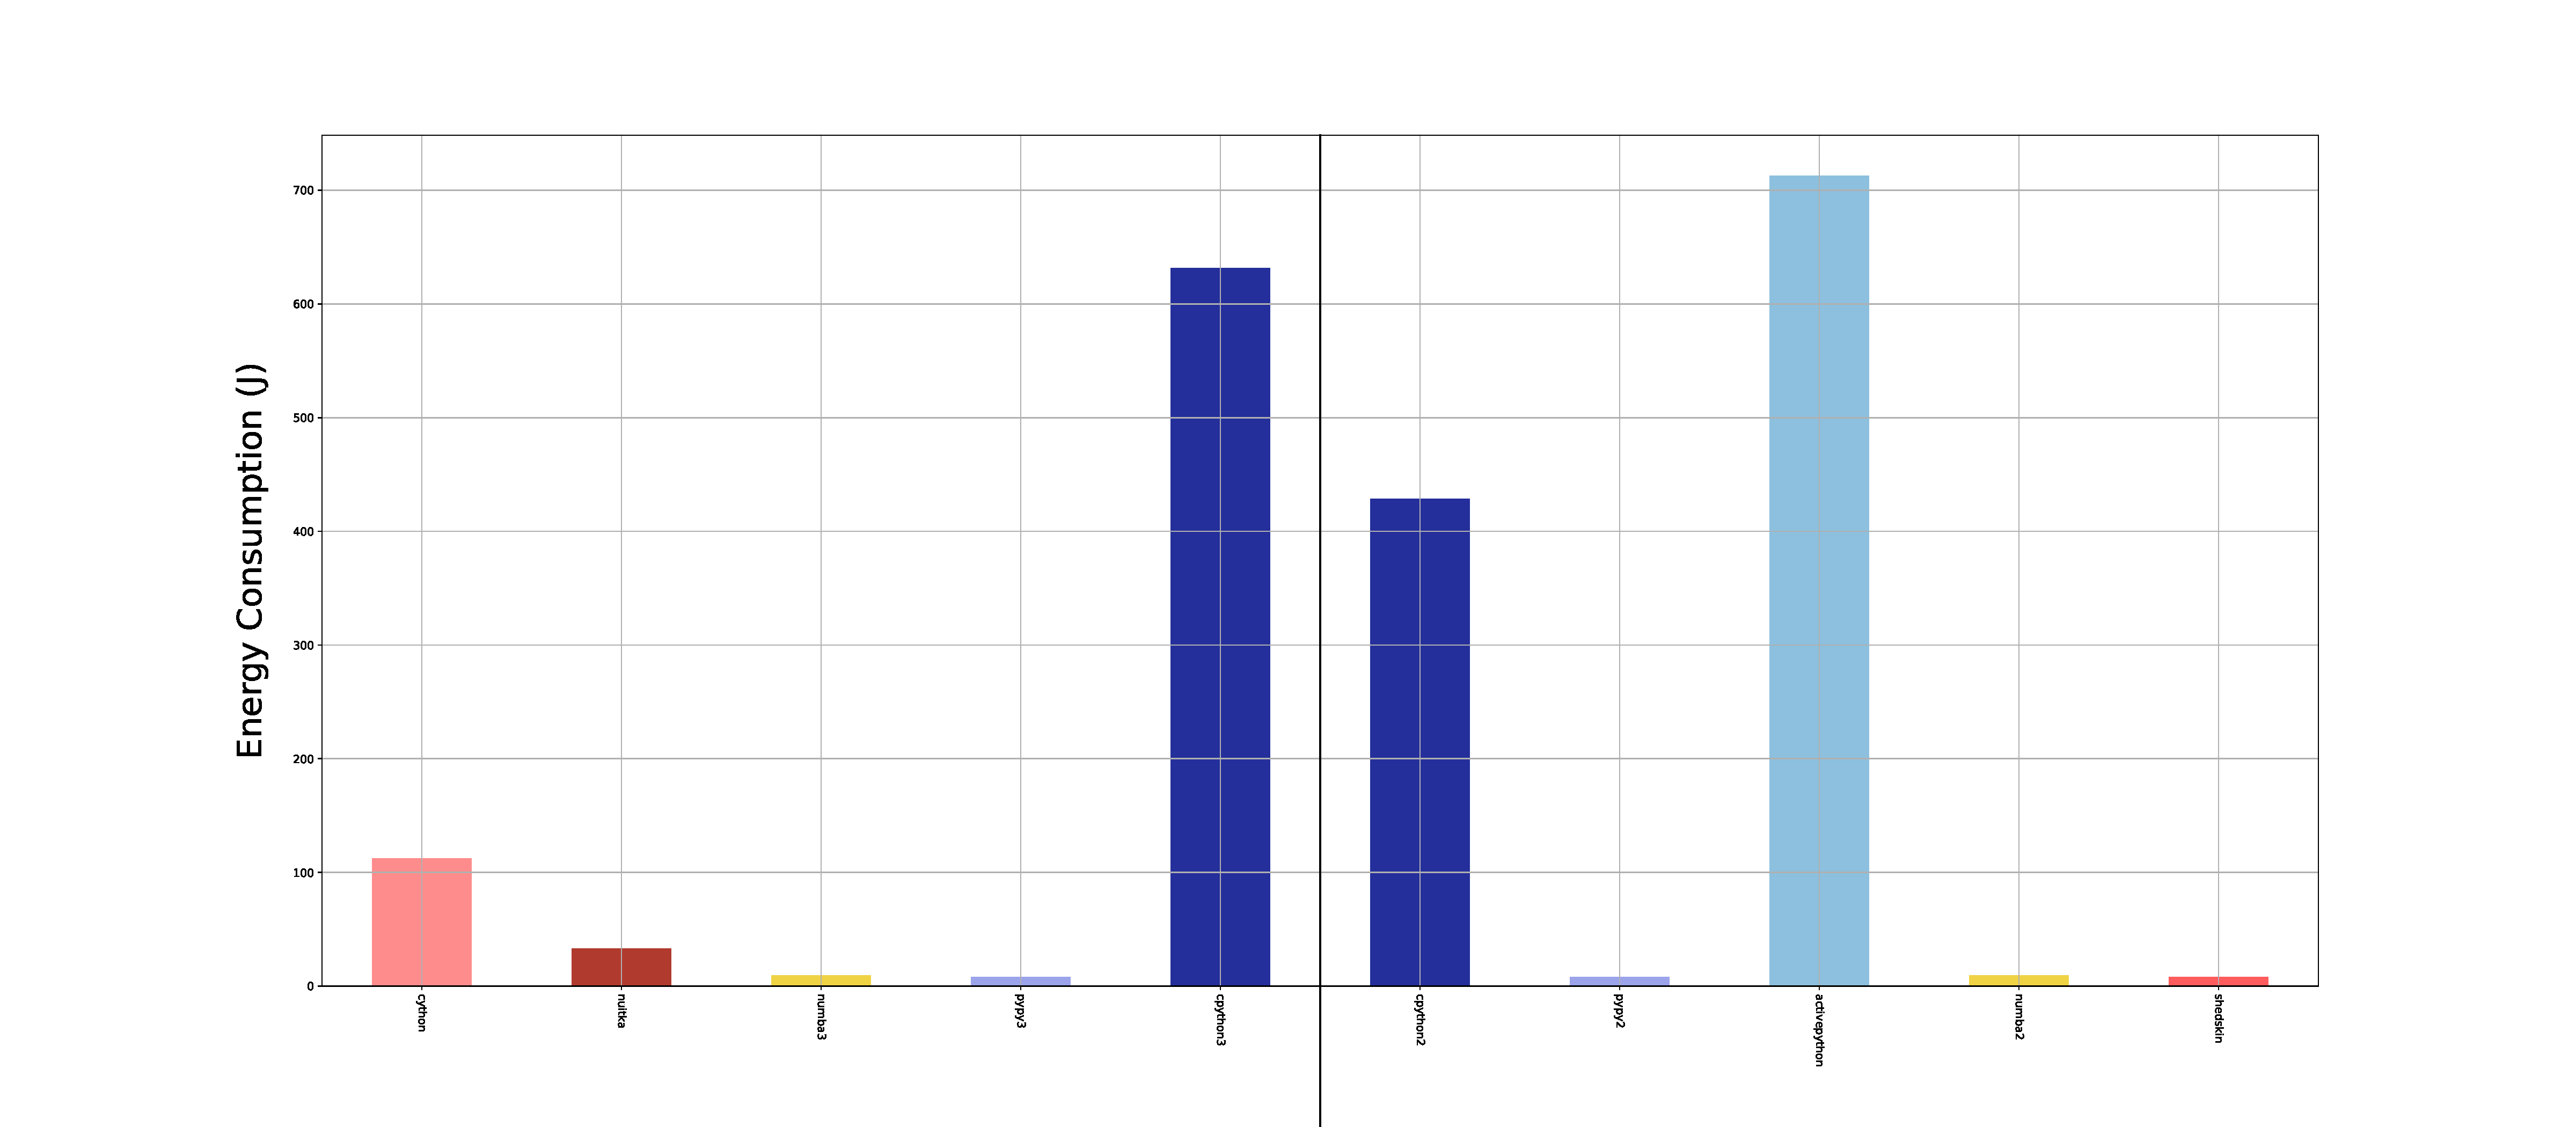
\includegraphics[width=\linewidth]{imgs/bitopts_mean}
    \caption{Mean consumption of different implementations of bit operations (Joule) }
    \label{fig:bitops}
\end{figure}

\begin{figure}
    \centering
    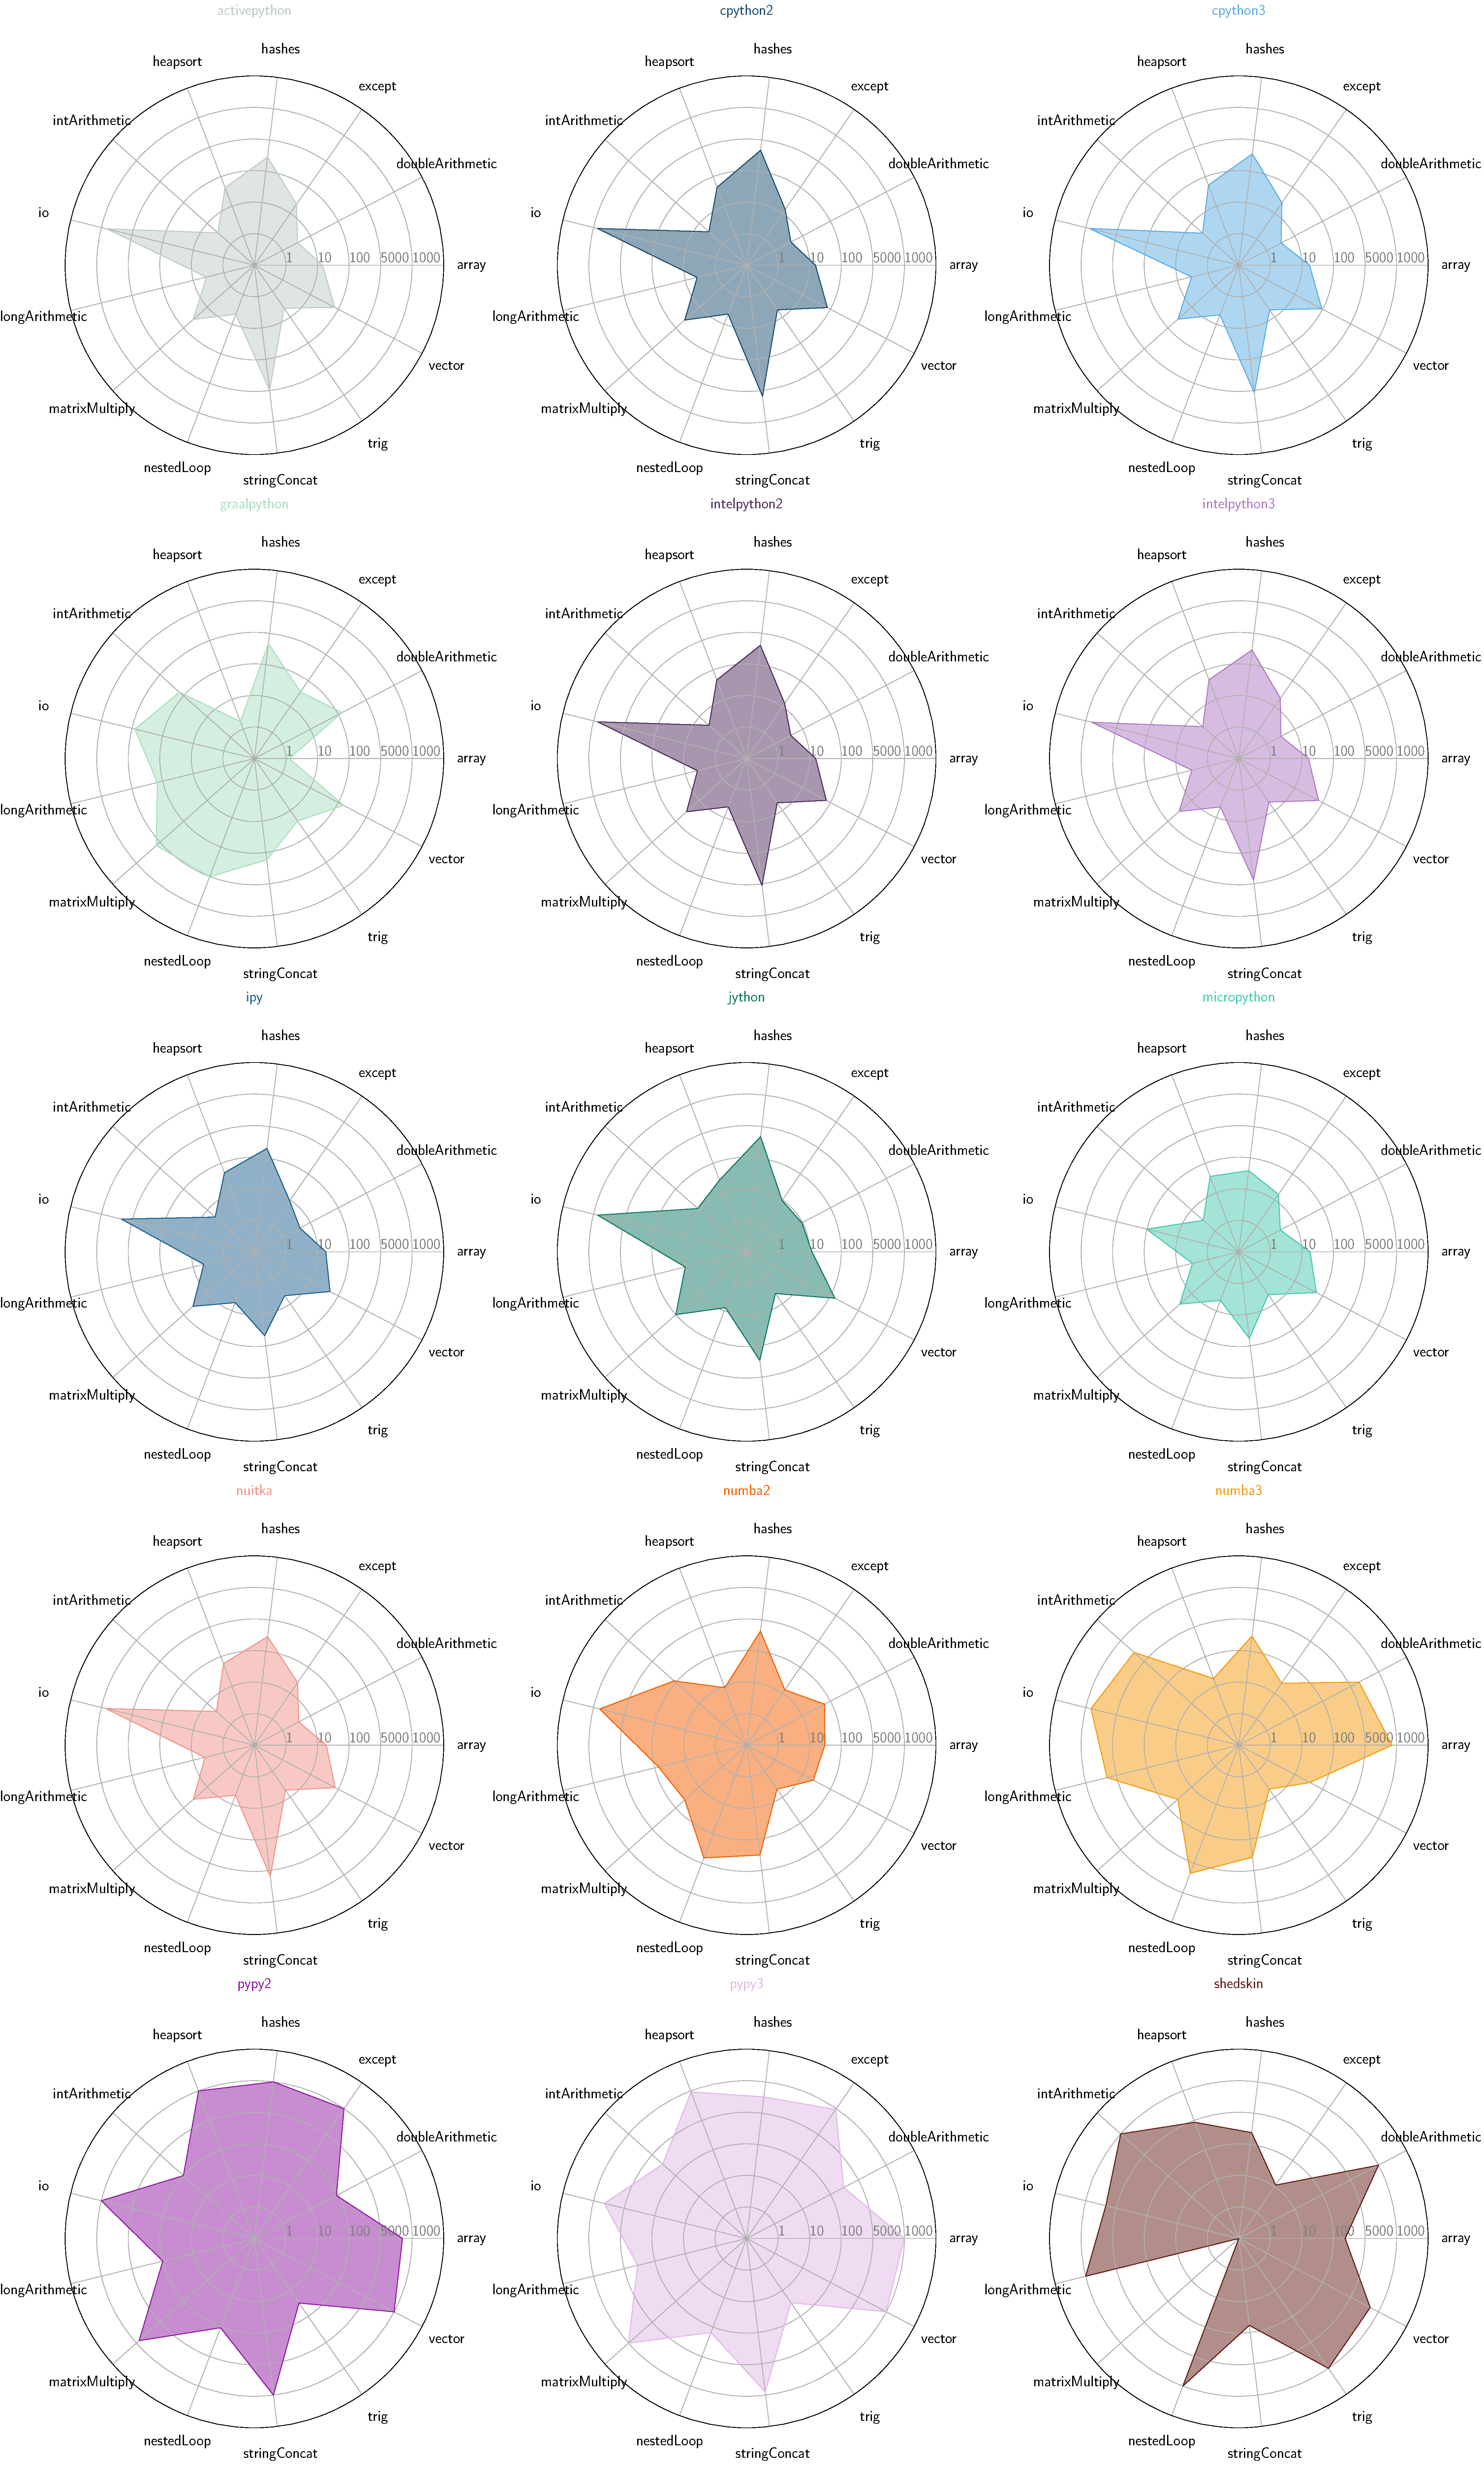
\includegraphics[width=\linewidth]{imgs/alltomti_performance}
    \caption{different interpererts optimisation }
    \label{fig:tommi_all}
\end{figure}
\begin{figure}
    \centering
    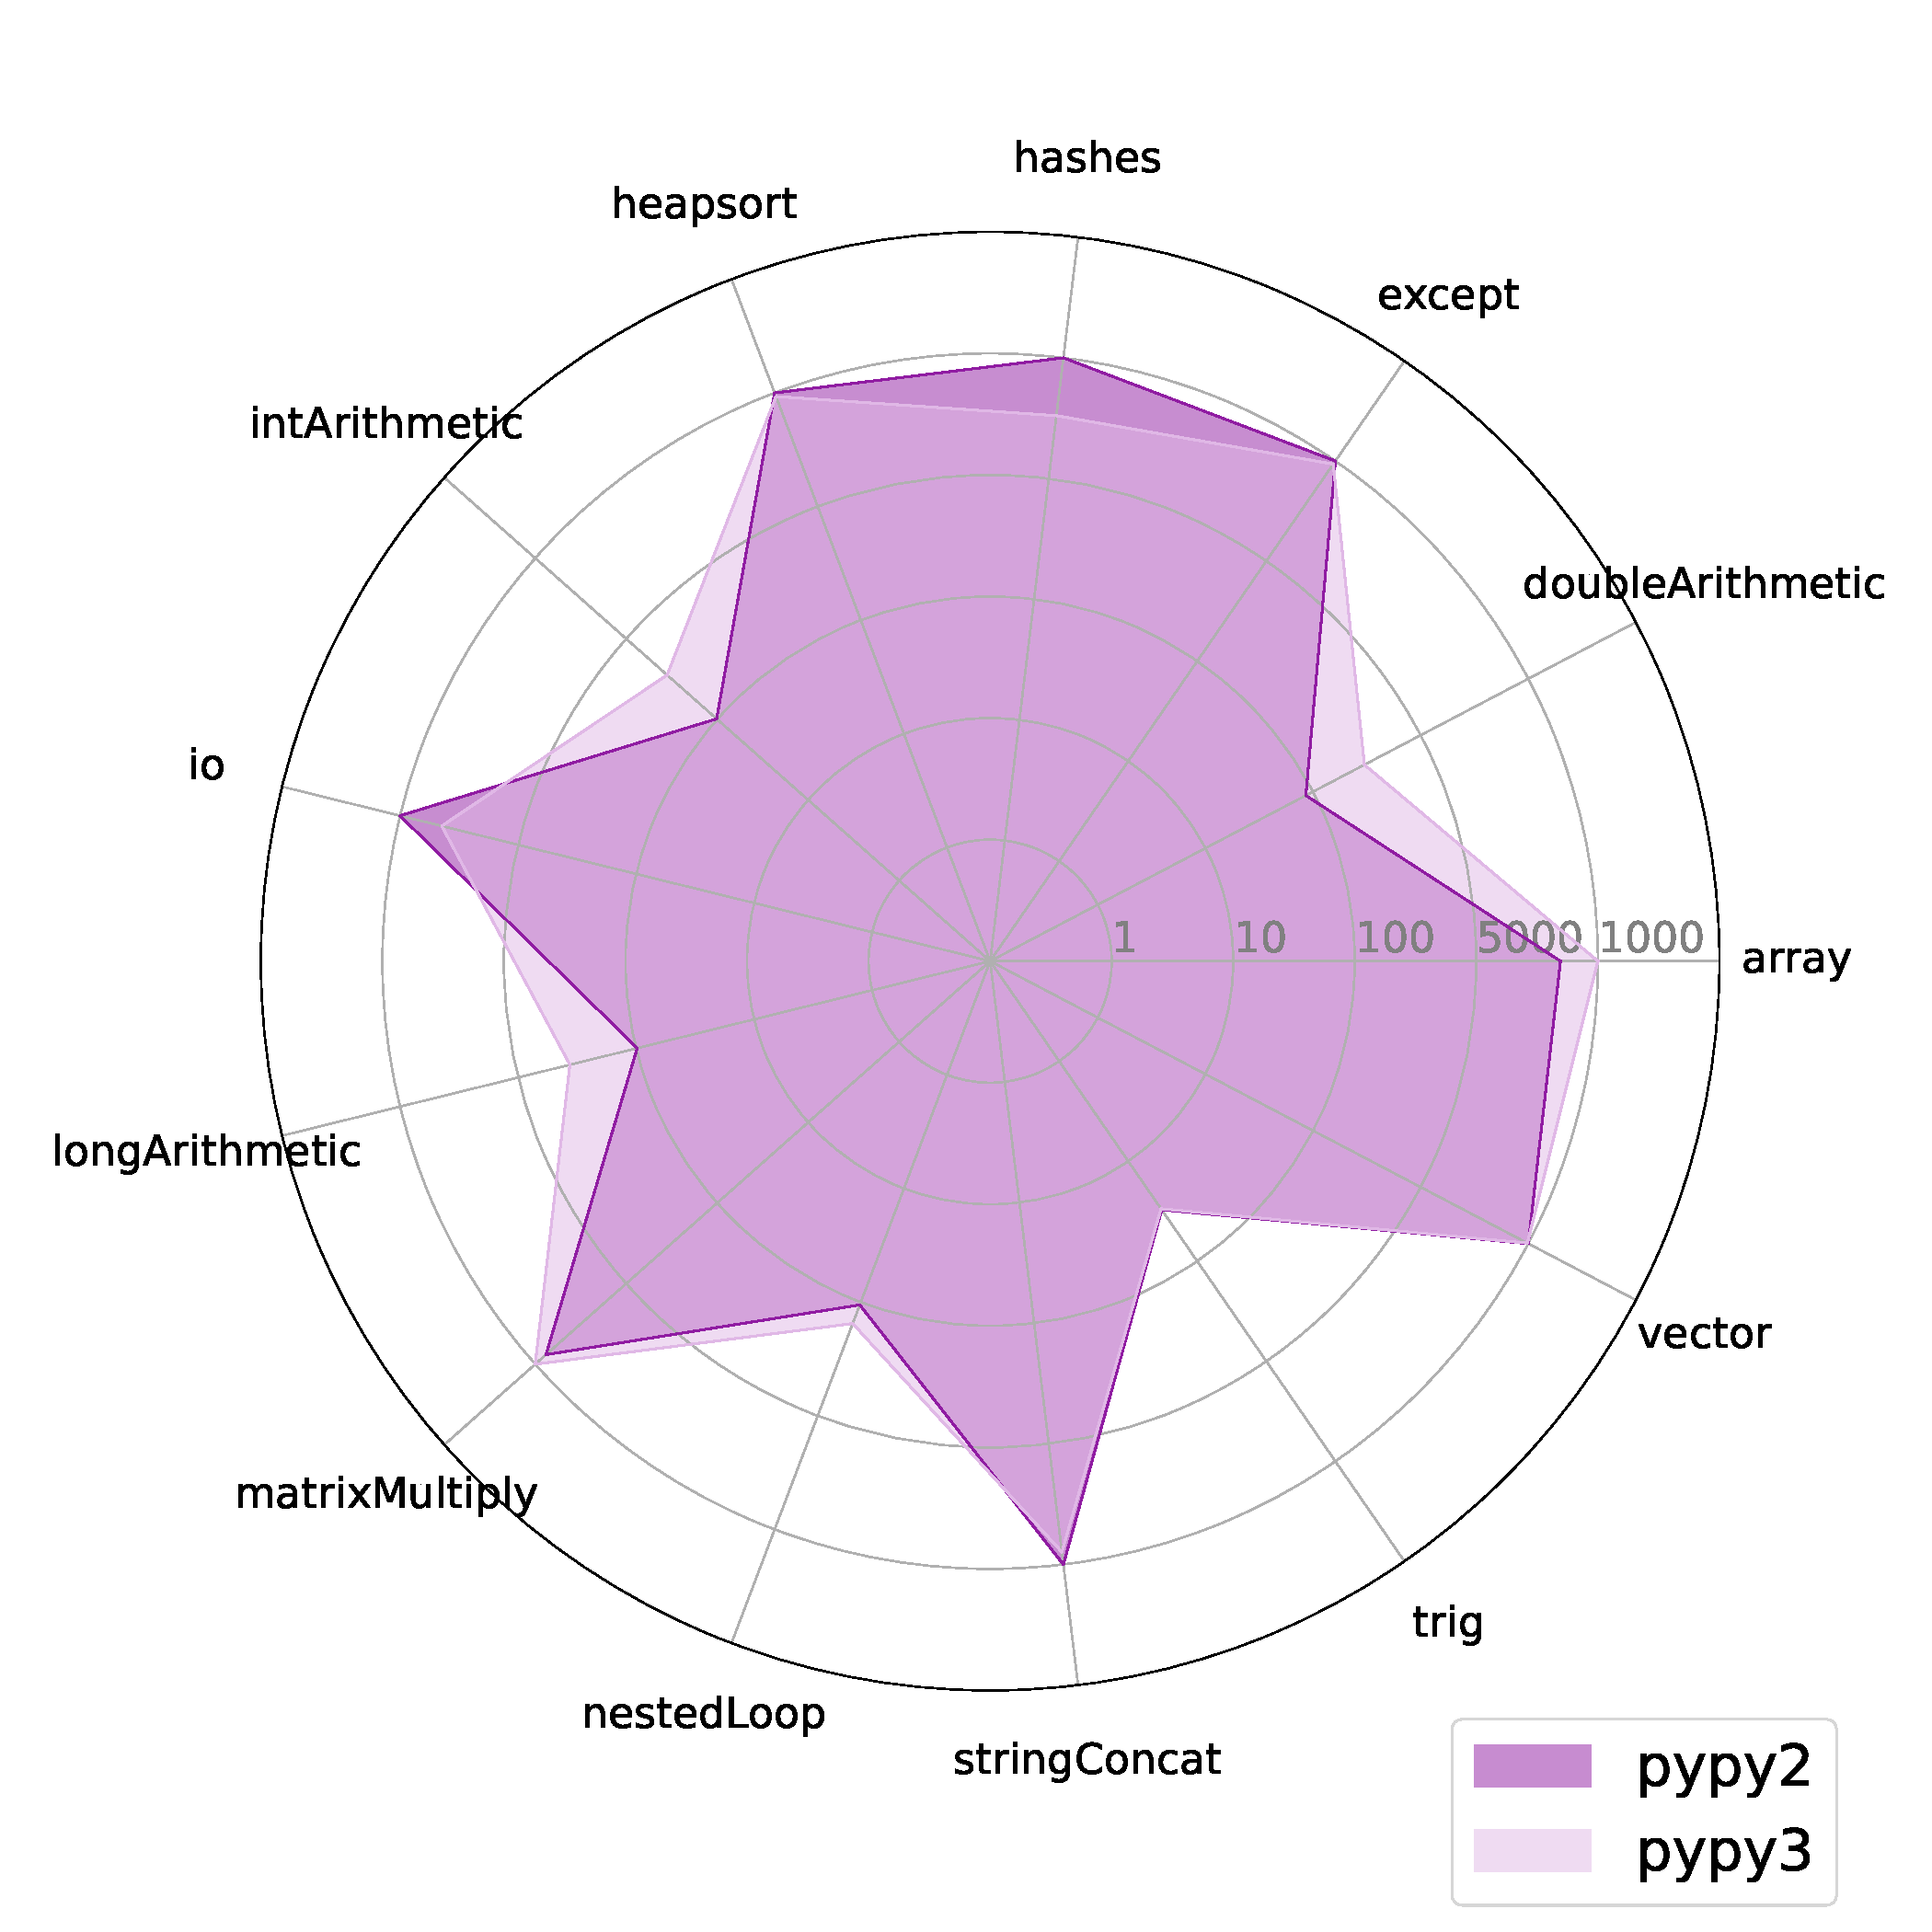
\includegraphics[width=\linewidth]{imgs/tommti_compare__pypy2_pypy3}
    \caption{green factor of pypy }
    \label{fig:pypy2vspypy3}
\end{figure}

\begin{figure}
    \centering
    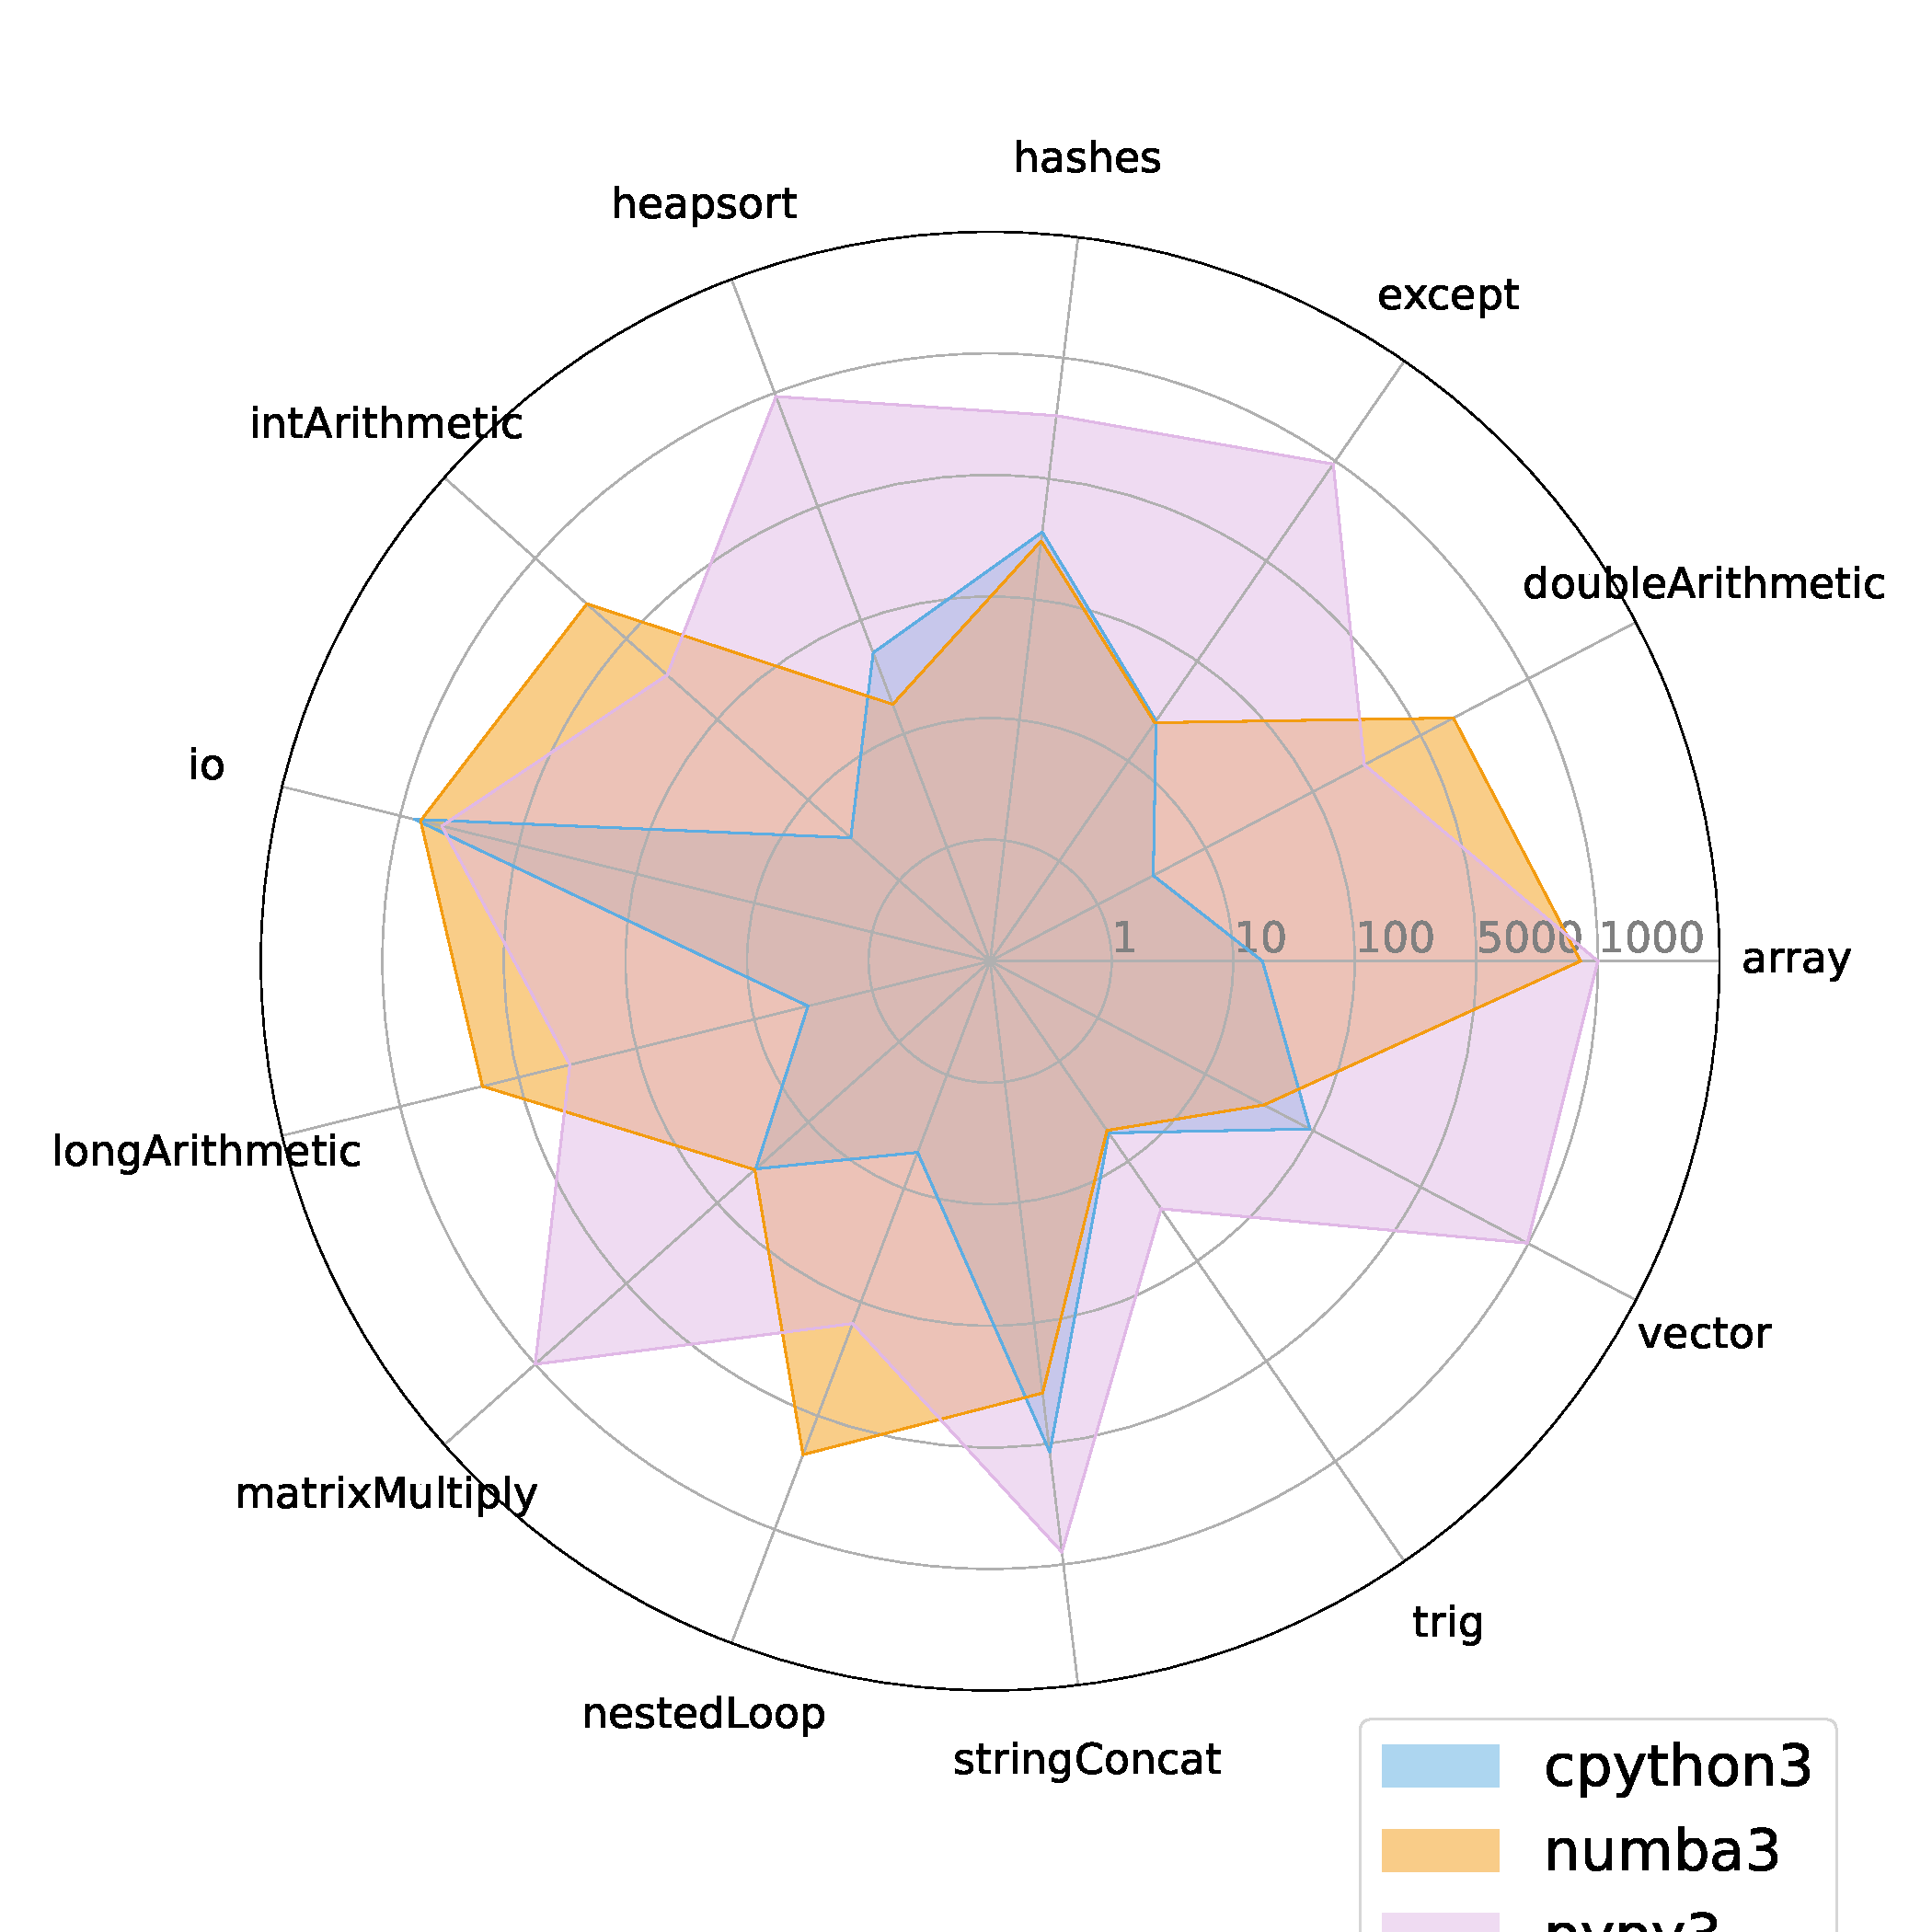
\includegraphics[width=\linewidth]{imgs/tommti_compare__cpython3_numba3_pypy3}
    \caption{comparaison of pypy vs python vs numba }
    \label{fig:p3}
\end{figure}

\begin{figure}
    \centering
    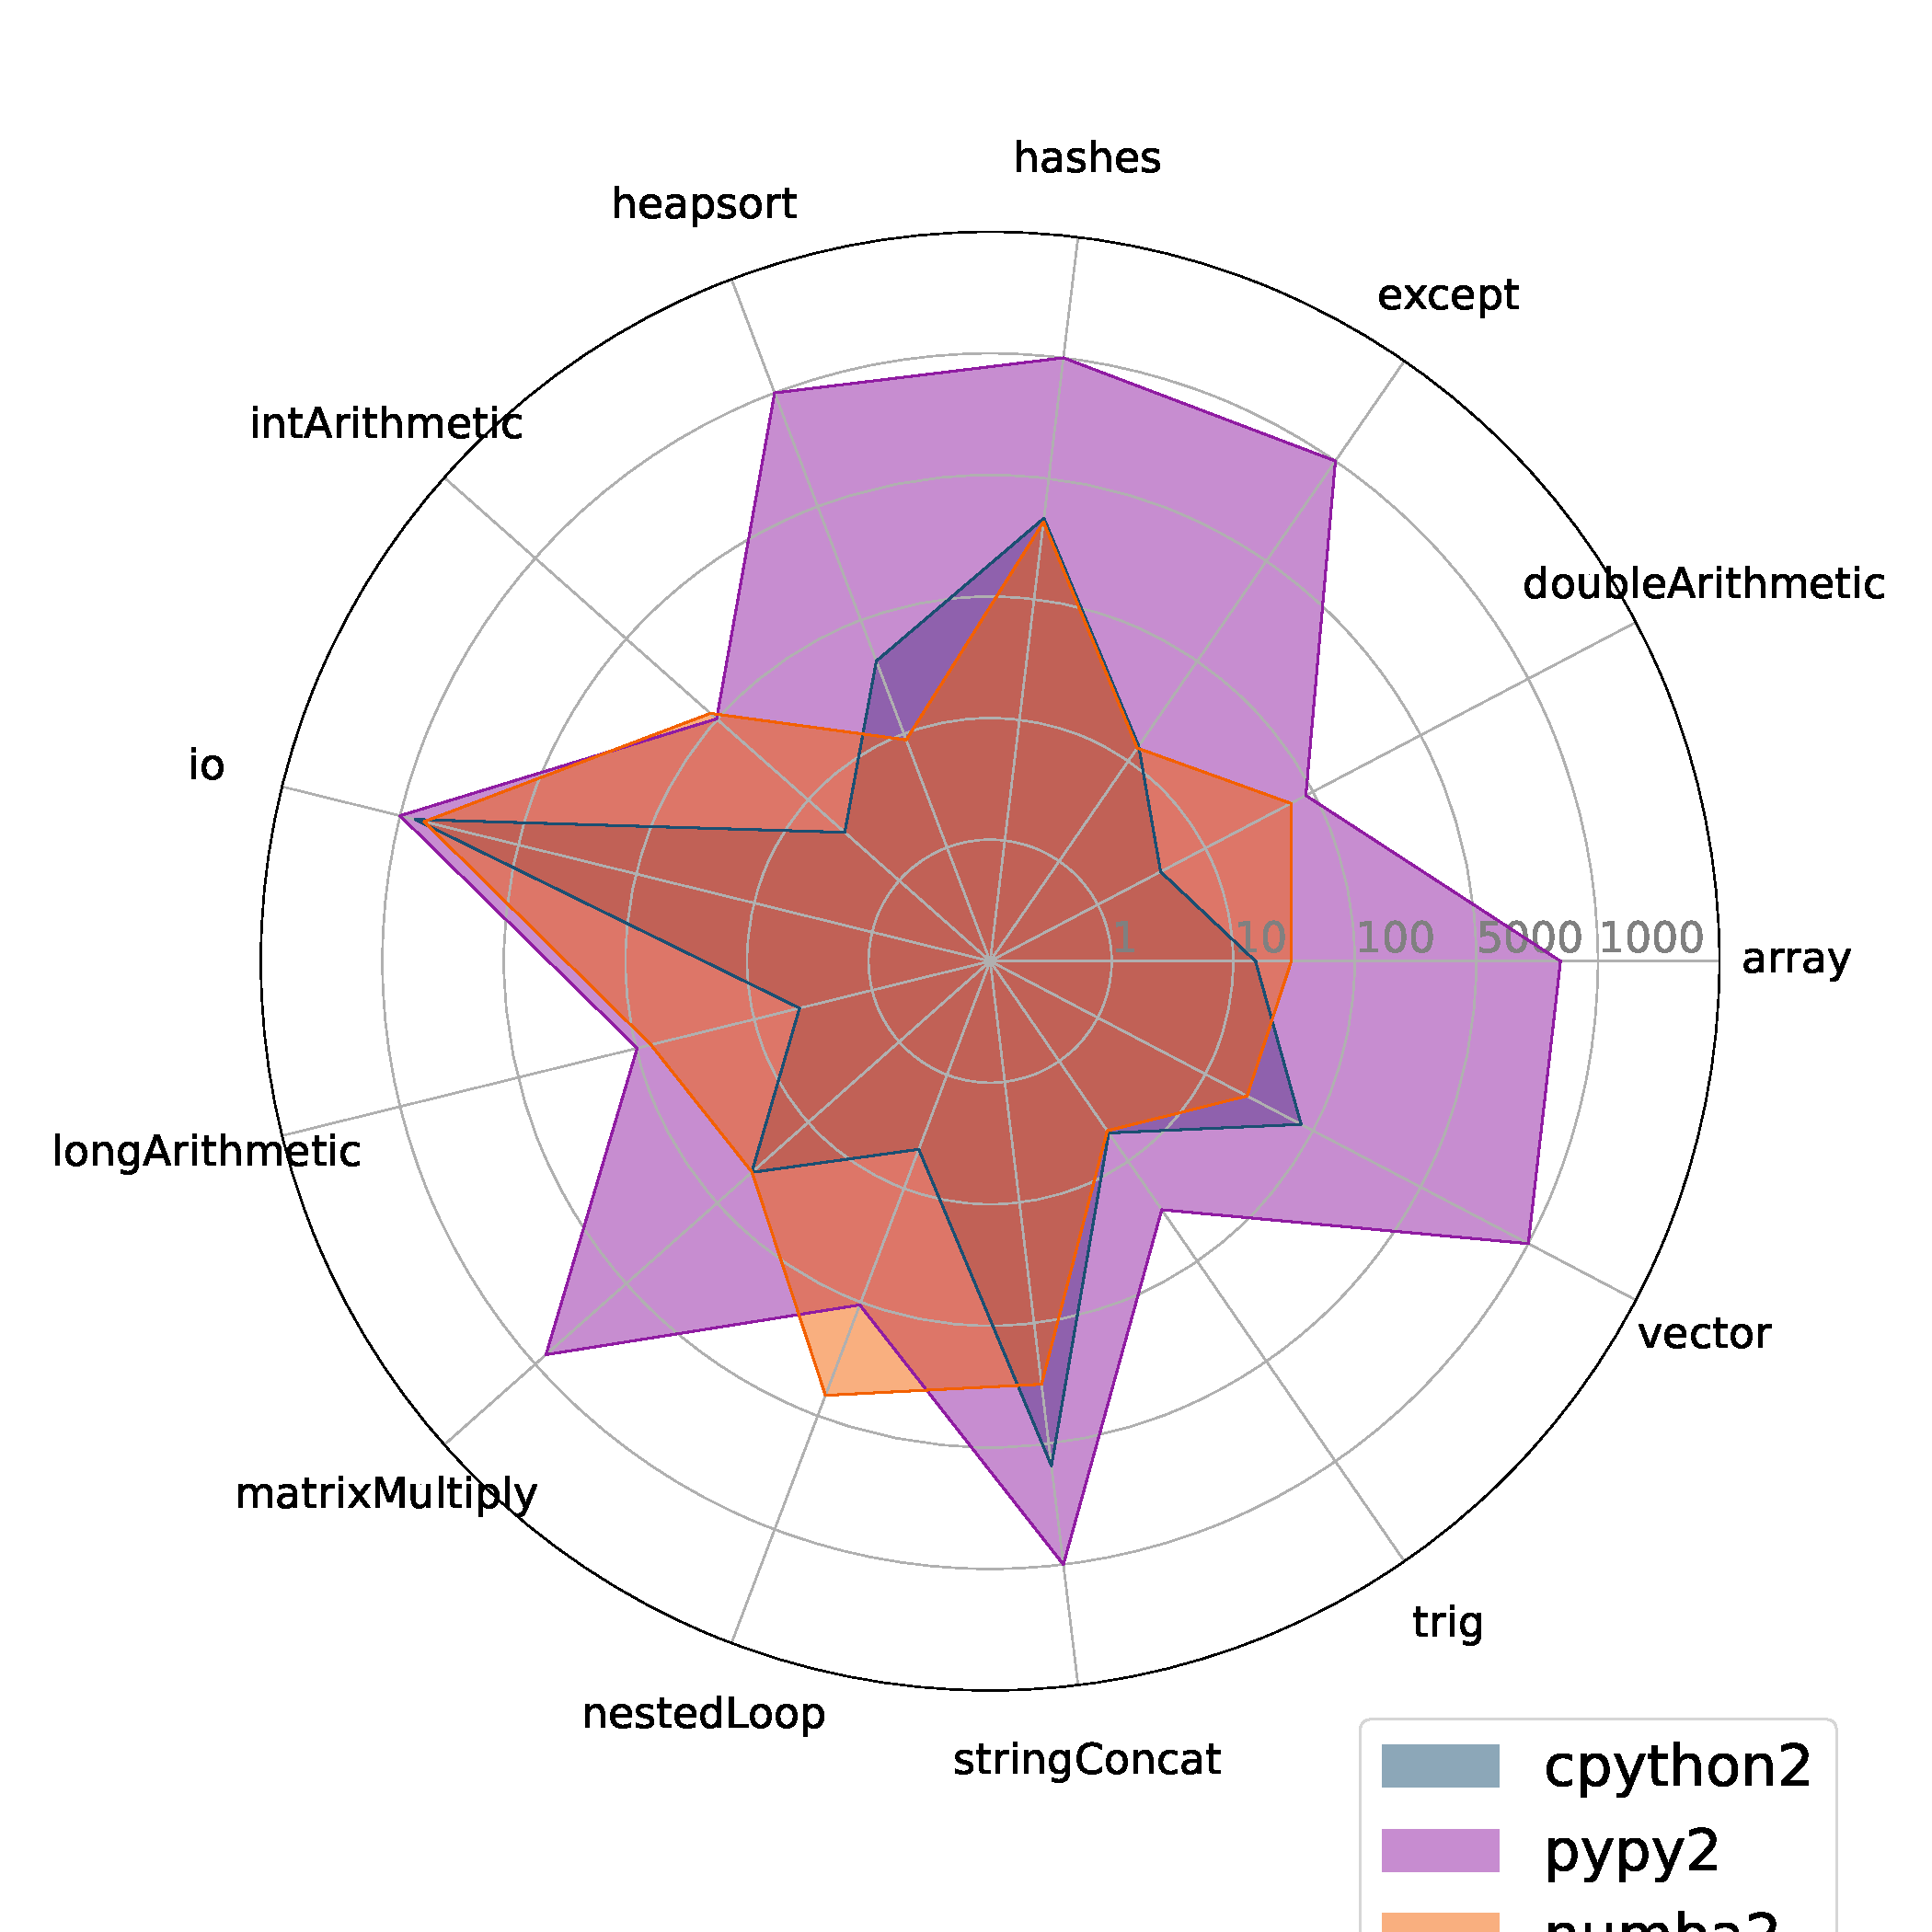
\includegraphics[width=\linewidth]{imgs/tommti_compare__cpython2_pypy2_numba2}
    \caption{comparaison of pypy vs python vs numba }
    \label{fig:p2}
\end{figure}

As we can see in figure \ref{fig:tommi_all}, there is no evolution between cpython2 and cpython3
Intelpython and active python both folows the same behaviour. one can conclude that the work that have been on those interpreters is mainly
to improve a specific purpose, Active python claims that their version is focused on secuirty which explains the lack of some performances due to the introduction of more reonforcment
.Morver Intel published their version of python as a dedicated for machine learning. Unfortunately the tommti benchmark is a set that focuses on the general purpose programming
which does not reflect the performance of the machine learning.
Another aspect of a such behaviour might be due to the fact of the processors that were used in the testbed. and it might change in the future if we include the GPU part for the machine learning benchmarks
% reference the work of the intern 
As for nuitka. there were no optimization in the energy consumpotion despite the fact that is it a complier.
However if we dig through the nuitka mechanisms. they basically embed the python code with an interpreter.
Unllike nuitka shedskin exhebit a the best energy consumption pattern when it comes to the arithmetic operartions. One can conclude it is due to the fact of the native type of the variables. unlike the interpreters where they are treated as object in the begining.

for the other interpeters pypy is very promising especially when it comes to data maniupulation as one can see in the figure \ref{fig:bar_tommti_vector}
pypy is by far the best interperer when it comes to treating vectors.
numba2 introduced the JIT but wasn't as promising as numba3.

for the other vm based interpereters. jython and ipy lacked in term of energy optimisation which was kinda expected since they were in their the begining of the stage and the main puprose of such implementation is to link the bytecode generated by jython and ironpython with their respectives virtual machin.

Unlike the the previous interpeters. graal exhebits a certin promises when it comes to complex algorithms - nested loops -
micro python is dedicated to embeded systems so lunching it is powerful cpu machines will be misleading.

Most of the interperters had the same behaviour when it comes to the input outputs. except for jython which was kinda of a anomaly probably due to the lack of the optimizations.
% pypy handles exceptions very well 


\section{conclusion}
One may observe that the choice of Python interpreter has a significant impact on the programs' energy consumption.
This investigation is made more intriguing by the absence of a universal solution.
The primary downside is the incompatibility of some of these solutions, which causes us to make concessions when we need a generic answer.



\begin{table*}

    \caption{Energy consumption python environment}
    \label{table:GC}
    \resizebox*{\linewidth}{!}{
        \begin{tabular}{l|rr|rr|rr|rr|rr|rr}
            \toprule

            Implementation & \multicolumn{2}{c}{array} & \multicolumn{2}{c}{intArithmetic} & \multicolumn{2}{c}{doubleArithmetic} & \multicolumn{2}{c}{hashes} & \multicolumn{2}{c}{heapsort} & \multicolumn{2}{c}{trig}                                                                                         \\
            \midrule

                           & energy (J)                & \em p-values                      & energy (J)                           & \em p-values               & energy (J)                   & \em p-values             & energy (J)     & \em p-values & energy (J) & \em p-values & energy (J) & \em p-values \\
            activepython   & 4e02                      & 0.0079                            & 6.9e02                               & 0.0022                     & 6.6e02                       & 0.0043                   & 9.7e02         & 0.0079       & 2.9e02     & 0.0079       & 5.1e02     & 0.0079       \\
            cpython2       & 3.4e02                    & 0.0079                            & 5.6e02                               & 0.0022                     & 5.5e02                       & 0.0043                   & 6.5e02         & 0.0079       & 2.9e02     & 0.0079       & 4.1e02     & 0.0079       \\
            cpython3       & 3.2e02                    & 0.0079                            & 7.4e02                               & 0.0022                     & 7.3e02                       & 0.0043                   & 7.9e02         & 0.0079       & 2.4e02     & 0.0079       & 4.1e02     & 0.0079       \\
            graalpython    & 1.2e05                    & 0.0079                            & 24                                   & 0.0022                     & 24                           & 0.0043                   & 6.4e02         & 0.0079       & 1.3e05     & 0.0079       & 72         & 0.0079       \\
            intelpython2   & 3.7e02                    & 0.0079                            & 5.9e02                               & 0.0022                     & 5.6e02                       & 0.0043                   & 7.1e02         & 0.0079       & 2.7e02     & 0.0079       & 4.2e02     & 0.0079       \\
            intelpython3   & 3.5e02                    & 0.0079                            & 7.7e02                               & 0.0022                     & 7.6e02                       & 0.0043                   & 9.4e02         & 0.0079       & 2.6e02     & 0.0079       & 4.8e02     & 0.0079       \\
            ipy            & 3e02                      & 0.0079                            & 4.4e02                               & 0.0022                     & 4.7e02                       & 0.0079                   & 1.3e03         & 0.0079       & 2.6e02     & 0.0079       & 4.5e02     & 0.0079       \\
            jython         & 5.2e02                    & 0.0079                            & 1.3e02                               & 0.0022                     & 1.6e02                       & 0.0043                   & 6.4e02         & 0.0079       & 4.6e02     & 0.0079       & 6.2e02     & 0.0079       \\
            micropython    & 3.1e02                    & 0.0079                            & 8.2e02                               & 0.0022                     & 8.4e02                       & 0.0079                   & 9.5e03         & 0.0079       & 3.4e02     & 0.0079       & 5.3e02     & 0.0079       \\
            nuitka         & 2.9e02                    & 0.0079                            & 5.4e02                               & 0.0022                     & 5.5e02                       & 0.0079                   & 9.5e02         & 0.0079       & 2.2e02     & 0.0079       & 3.9e02     & 0.0079       \\
            numba2         & 1.9e02                    & 0.0079                            & 27                                   & 0.0022                     & 36                           & 0.0079                   & 6.8e02         & 0.0079       & 2.1e03     & 0.0079       & 4.4e02     & 0.0079       \\
            numba3         & \best{11}                 & \best{best}                       & 10                                   & 0.0022                     & 10                           & 0.0079                   & 9.1e02         & 0.0079       & 7.2e02     & 0.0079       & 4.5e02     & 0.0079       \\
            pypy2          & 16                        & \same{0.15}                       & 29                                   & 0.0022                     & 30                           & 0.0043                   & \best{ 1.1e02} & \best{best}  & \best{20}  & \best{best}  & 64         & 0.0079       \\
            pypy3          & 13                        & \same{0.15}                       & 17                                   & 0.0022                     & 18                           & 0.0079                   & 1.9e02         & 0.0079       & \best{20}  & 0.31         & 65         & 0.0079       \\
            shedskin       & 47                        & 0.0079                            & \best{7.4}                           & \best{best}                & \best{7.3 }                  & \best{best}              & 1.1e03         & 0.0079       & 44         & 0.0079       & \best{7.7} & \best{best}  \\
            \bottomrule
        \end{tabular}

    }
    \vfill
    \resizebox*{\linewidth}{!}{
        \begin{tabular}{l|rr|rr|rr|rr|rr|rr}

            Implementation & \multicolumn{2}{c}{longArithmetic} & \multicolumn{2}{c}{matrixMultiply} & \multicolumn{2}{c}{io} & \multicolumn{2}{c}{stringConcat} & \multicolumn{2}{c}{nestedLoop} & \multicolumn{2}{c}{except}                                                                                     \\
            \midrule
                           & energy (J)                         & \em p-values                       & energy (J)             & \em p-values                     & energy (J)                     & \em p-values               & energy (J) & \em p-values & energy (J) & \em p-values & energy (J) & \em p-values \\
            activepython   & 6.7e02                             & 0.0079                             & 4.3e02                 & 0.0079                           & 2.1e02                         & 0.0079                     & 14         & 0.0079       & 4.1e02     & 0.0079       & 2.6e02     & 0.0079       \\
            cpython2       & 5.5e02                             & 0.0079                             & 4e02                   & 0.0079                           & 2e02                           & 0.0079                     & 12         & 0.0079       & 4.2e02     & 0.0079       & 4.3e02     & 0.0079       \\
            cpython3       & 7.4e02                             & 0.0079                             & 4.4e02                 & 0.0079                           & 2e02                           & 0.0079                     & 13         & 0.0079       & 3.8e02     & 0.0079       & 2.3e02     & 0.0079       \\
            graalpython    & 24                                 & 0.0079                             & 45                     & 0.0079                           & 7.5e02                         & 0.0079                     & 26         & 0.0079       & 12         & 0.0079       & 1.6e02     & 0.0079       \\
            intelpython2   & 5.7e02                             & 0.0079                             & 4.8e02                 & 0.0079                           & 2e02                           & 0.0079                     & 13         & 0.0079       & 4.4e02     & 0.0079       & 4.6e02     & 0.0079       \\
            intelpython3   & 7.7e02                             & 0.0079                             & 5e02                   & 0.0079                           & 2.2e02                         & 0.0079                     & 14         & 0.0079       & 4.4e02     & 0.0079       & 2.7e02     & 0.0079       \\
            ipy            & 4.7e02                             & 0.0079                             & 4.1e02                 & 0.0079                           & 3.8e02                         & 0.0079                     & 49         & 0.0079       & 3.3e02     & 0.0079       & 7.2e02     & 0.0079       \\
            jython         & 1.6e02                             & 0.0079                             & 1.9e02                 & 0.0079                           & 2e02                           & 0.0079                     & 21         & 0.0079       & 1.9e02     & 0.0079       & 7.1e02     & 0.0079       \\
            micropython    & 8.3e02                             & 0.0079                             & 5.3e02                 & 0.0079                           & 5.3e03                         & 0.0079                     & 44         & 0.0079       & 4.3e02     & 0.0079       & 3.6e02     & 0.0079       \\
            nuitka         & 5.4e02                             & 0.0079                             & 4.3e02                 & 0.0079                           & 2e02                           & 0.0079                     & 12         & 0.0079       & 3.6e02     & 0.0079       & 2.2e02     & 0.0079       \\
            numba2         & 35                                 & 0.0079                             & 4e02                   & 0.0079                           & 2.2e02                         & 0.0079                     & 20         & 0.0079       & 14         & 0.0079       & 4.5e02     & 0.0079       \\
            numba3         & 11                                 & 0.0079                             & 4.2e02                 & 0.0079                           & 2.1e02                         & 0.0079                     & 19         & 0.0079       & 10         & 0.0079       & 2.4e02     & 0.0079       \\
            pypy2          & 30                                 & 0.0079                             & 24                     & 0.056                            & \best{1.7e02}                  & \best{best}                & 7.7        & \best{best}  & 27         & 0.0079       & \best{14}  & \best{best}  \\
            pypy3          & 17                                 & 0.0079                             & \best{23}              & \best{best}                      & 2.6e02                         & 0.0079                     & 8.3        & 0.69         & 23         & 0.0079       & 14         & 0.69         \\
            shedskin       & \best{7.8}                         & \best{best}                        &                        &                                  & 3.8e02                         & 0.0079                     & 44         & 0.0079       & 7.1        & \best{best}  & 5.6e02     & 0.0079       \\

            \bottomrule
        \end{tabular}
    }

\end{table*}

